\documentclass[11pt]{article}

\usepackage[utf8]{inputenc}
\usepackage[top=1in, bottom=1in, left=1in, right=1in]{geometry}
\usepackage{graphicx}
\usepackage{enumitem}
\usepackage[table]{xcolor}
\usepackage{color}
\usepackage{hyperref}

\usepackage{listings}

\usepackage{subcaption}

\definecolor{dkgreen}{rgb}{0,0.6,0}
\definecolor{gray}{rgb}{0.5,0.5,0.5}
\definecolor{mauve}{rgb}{0.58,0,0.82}

\lstset{frame=tb,
  language=xml,
  aboveskip=3mm,
  belowskip=3mm,
  showstringspaces=false,
  columns=flexible,
  basicstyle={\small\ttfamily},
  numbers=none,
  numberstyle=\tiny\color{gray},
  keywordstyle=\color{blue},
  commentstyle=\color{dkgreen},
  stringstyle=\color{mauve},
  breaklines=true,
  breakatwhitespace=true,
  tabsize=3
}

\hypersetup{
  colorlinks=true,
    linkcolor=black,
    filecolor=magenta,      
    urlcolor=cyan,
}

\begin{document}

\title{\begin{Huge} Essential Skills \end{Huge}}
  \author{\begin{Large} Max Grim, Alexander Blaauwgeers, Marwin Baumann and Vincent van Dongen \end{Large}}
    \date{\today}
\maketitle

\begin{center}
  Homework group 2\\[1in]
  
\includegraphics[scale=1.5]{uva.png}
  {\begin{huge} \LaTeX \ assignment \end{huge}}
\end{center}

\newpage
\tableofcontents

\newpage
\section{Introduction}
In this document we highlight to assignment of the course \textit{essential skills}. Below, you can find the \textbf{Assignment Review Process}.

\subsection{Assignment Review Process}

To help you prepare your assignment here are a couple of points:
\begin{itemize}
  \item \textbf{Feedback} is given on a weekly basis
    \begin{itemize}
      \item To get feedback you have to finish your assignment before the deadline (announced by the lab teachers).
      \item You will receive the feedback usually one week after the deadline.
      \item If you miss a deadline you will get feedback somewhere before the end of the block.
      \item At the end of the block the lab teachers will determine whether your assignments were sufficient. They must be sufficient for you to pass the course.
    \end{itemize}
  \item The \textbf{group assignment}
    \begin{itemize}
      \item A kind of homework with the objective to work in a group (to get to know your classmates) and learn a bit more about a given topic.
      \item It consists of reading a paper or watching an online video (Keynotes, tutorials, lectures, …)
      \item TO DO:
        \begin{itemize}
          \item extract the interesting points and write a short summary on your own wiki (Text, figures, references …)
          \item discuss them with you group members
          \item Present them in the next lecture (2 to 3 min per group, so be prepared)
        \end{itemize}
    \end{itemize}
  \item \textbf{How we review your assignments}: following criteria are important
    \begin{itemize}
      \item clarity of the given explanations
      \item references
      \item analysis of the proposed further reading (HomeWork)
      \item robustness of the proposed solution (programming, regular expression)
      \item comments
      \item presentation and layout
    \end{itemize}
\end{itemize}

\newpage

\section{Assignments}
Below, you can find the progress for the group assignments. We have created a table to provide you a complete overview:

\begin{center}
  \rowcolors{1}{lightgray}{white}
  \begin{tabular}{| c | c | c | c |}
    \hline
    \textbf{number} & \textbf{Assignment} & \textbf{Status}  \\ \hline
    1a & Assignment 1 : WIKI, XML and CSS & \textcolor{green}{Completed}  \\ \hline
    1b & Assignment 1 : WIKI, XML and CSS & \textcolor{green}{Completed}  \\ \hline
    2 & Assignment 2 : Regular expressions & \textcolor{green}{Completed}  \\ \hline
    3 & Assignment 3 : Text Editing Tools & \textcolor{green}{Completed} \\ \hline
    4 & Assignment 4 : Build tools & \textcolor{green}{Completed} \\ \hline
    5 & Assignment 5 : Version Control Systems & \textcolor{yellow}{Pending} \\ \hline
    6 &     Assignment 6 : Latex & \textcolor{orange}{started} \\ \hline
    7 & assignment 7 & \textcolor{red}{Expected} \\ \hline
    8 & assignment 8 & \textcolor{red}{Expected}  \\ \hline
    9 & assignment 9 & \textcolor{red}{Expected}  \\ \hline
    10 & assignment 10 & \textcolor{red}{Expected}  \\ \hline
    11 & assignment11 & \textcolor{red}{Expected}  \\
    \hline
  \end{tabular}
\end{center}

\subsection{Team members}
The group consist of 4 people:
\begin{enumerate}
  \item Max Grim
  \item Alexander Blaauwgeers
  \item Marwin Baumann
  \item Vincent van Dongen 
\end{enumerate}

\newpage
\subsection{Photo's}
Below, you can see the photo's

\begin{figure}[htbp]
  \begin{minipage}[b]{0.25\linewidth}
    \centering
    
\includegraphics[width=0.9\linewidth]{max.jpg}
    \caption{Max Grim}
  \end{minipage}
  \hspace{6.0cm}
  \begin{minipage}[b]{0.25\linewidth}
    \centering
    
\includegraphics[width=1.1\linewidth]{marwin.jpg}
    \caption{Marwin Baumann}
  \end{minipage}
\end{figure}

\begin{figure}[htbp]
  \begin{minipage}[b]{0.25\linewidth}
    \centering
    
\includegraphics[width=1.5\linewidth]{blaauwgeersba.jpg}
    \caption{Alexander Blaauwgeers}
  \end{minipage}
  \hspace{6.0cm}
  \begin{minipage}[b]{0.25\linewidth}
    \centering
    
\includegraphics[width=1.2\linewidth]{vin.png}
    \caption{Vincent van Dongen}
  \end{minipage}
\end{figure}

\newpage
\section {The first week: \textit{Atom}}
Atom consists of two web standards and is developed as an alternative to RSS. The Atom Publishing Protocol is based on HTTP and provides a standardized way to export/back-up structured data, like blogs, and the Atom Syndication Format (RFC 4287) (further called Atom) is serialized as XML 1.0 language, and is used for web feeds (similar to RSS). Web feeds can be used for activity involving periodic updates or publications; e.g. by the blogging community, journalists, bug-reporters \cite{source1}. The specification is structured such that further versions/revisions can be released without breaking earlier specifications/implementations \cite{source1,source2}. 

There are two kinds of Atom Documents: Atom Feed Documents and Atom Entry Documents.

\subsection{Feed Document}
An Atom Feed Document is a representation of an Atom feed, including metadata about the feed, and some or all of the entries associated with it. \cite{source3} An Atom Feed Document requires the following feed elements:
\begin{lstlisting}
id:    Identifies the feed using a universally unique and permanent URI  
title:    Contains a human readable title for the feed.                 
update: Indicates the last time the feed was modified in a significant way.
\end{lstlisting}

\subsection{Entry Document}
An Atom Entry Document represents exactly one Atom entry, outside of the context of an Atom feed. Its root is the atom:entry element. An Atom Entry Document requires the following entry elements:
\begin{lstlisting}
author:     Names one author of the entry.
content: Contains or links to the complete content of the entry. 
link:       Identifies a related Web page.
summary: Conveys a short summary, abstract, or excerpt of the entry. 
\end{lstlisting}

\begin{figure}[htbp]
  \begin{minipage}[b]{0.7\linewidth}
    \centering
    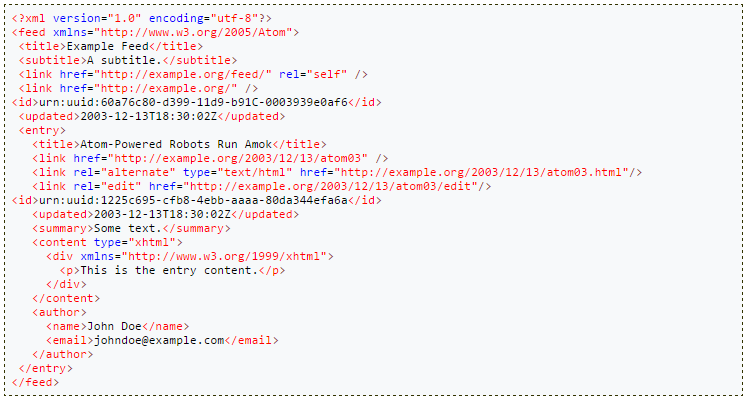
\includegraphics[width=0.9\linewidth]{Capture.png}
    \caption{source code}
    \label{fig:chapter001_dist_001}
  \end{minipage}
\end{figure}

\newpage

\section {The second week: \textit{XPath}}
\begin{itemize}
  \item XPath is a syntax for selecting nodes in a XML document.
  \item XPath uses path expressions to navigate in XML documents.
  \item XPath contains a library of standard functions.
  \item XPath is part of the \href{https://www.w3.org/TR/xslt}{W3C XSLT standard}.
\end{itemize}  

\textbf{Terminology}

XML documents are treated as trees of nodes. The topmost element of the tree is called the root element \cite{w3c1}.

\begin{lstlisting}
<?xml version="1.0" encoding="UTF-8"?>

<bookstore> <!-- root element node -->
  <book> <!-- element node -->
    <title lang="en">Harry Potter</title> <!-- lang="en" => attribute node -->
    <author>J K. Rowling</author> <!-- element node -->
    <year>2005</year> <!-- element node -->
    <price>29.99</price> <!-- element node -->
  </book>
</bookstore>
\end{lstlisting}

\textbf{XPath Expressions}
XPath expressions are used to query certain objects inside an XML document. This can be useful for example to find the right collection of books inside a big XML dataset based on a query \cite{xpathwiki}.

Select a node:

\begin{itemize}
  \item From root: /
  \item Relative: //
  \item Attribute: @
\end{itemize}

\textbf{Predicates}
\begin{itemize}
  \item are used to find a specific node/value.
  \item embedded in []
\end{itemize}

\underline{Example:} 

Select the first edition of each book.

\begin{lstlisting}
collection/books/book/editions/edition/*[1]
\end{lstlisting}

Select all the atlases.

\begin{lstlisting}
collection/books/book[@name="Atlas"]/editions/edition/*
\end{lstlisting}

bookcollection.xml

\begin{lstlisting}
<?xml version="1.0" encoding="utf-8"?>
<collection>
  <books>
    <book name="Dictionary">
      <editions>
        <edition>English</edition>
        <edition>Dutch-English</edition>
        <edition>English-Dutch</edition>
        <edition>Dutch</edition>
      </editions>
    </book>
    <book name="Atlas">
      <editions>
        <edition>Netherlands</edition>
        <edition>Europe</edition>
        <edition>Asia</edition>
        <edition>Australia</edition>
      </editions>
    </book>
  </books>
</collection>
\end{lstlisting}

\textbf{Functions}
There are over 100 functions in XPath. Eg. for numeric values, string values, date and time, sequence manipulation, Boolean values, and more.

It is also possible to compute values. This includes operations such as
\begin{itemize}
  \item addition (+)
  \item subtraction (-)
  \item multiplication (*).
  \item etc..
\end{itemize}

Additionally conditions such as

\begin{itemize}
  \item Equal { = }
  \item less than { < }
  \item  and { and }
  \item or { or }
  \item etc..
\end{itemize}

and so forth can be specified inside the path expressions.

\newpage
\section {The third week: \textit{Regex}}
\subsection{Lazy and Greedy quantifier in Regex}
Greedy RegEx will consume as much text as possible, whereas Lazy Regex will repeat as few times as possible (match the shortest possible string). \\

\textbf{Example (greedy):} \\
We want to match $<$em$>$ and $<$/em$>$ in the following string: $<$em$>$Hello World$<$/em$>$:

\begin{itemize}
  \item Lets use: $<$.+$>$.
  \item Will this only match the $<$em$>$ and $<$/em$>$?
  \item No!
  \item The RegEx will be very Greedy and will match from the first $<$ to the last $>$.
  \item Result: RegEx will match: $<$em$>$Hello World$<$/em$>$
\end{itemize}

\textbf{Let's make the RegEx lazy:}
\begin{itemize}
  \item Lets use: $<$.+?$>$
  \item Will this only match the $<$em$>$ and $<$/em$>$?
  \item Yes!
  \item By adding the ? after the +, we want the RegEx to repeat as few times as possible, so the first $>$ it comes across, is where we want to stop the matching.
\end{itemize}

The examples of both regular expressions are illustrated in Figure \ref{fig:regexes}.

\begin{figure}[b]
  \centering
  \begin{subfigure}{.5\textwidth}
    \centering
    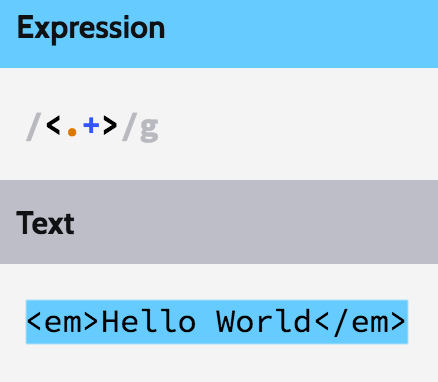
\includegraphics[width=.4\linewidth]{expr1}
    \caption{Greedy}
  \end{subfigure}%
  \begin{subfigure}{.5\textwidth}
    \centering
    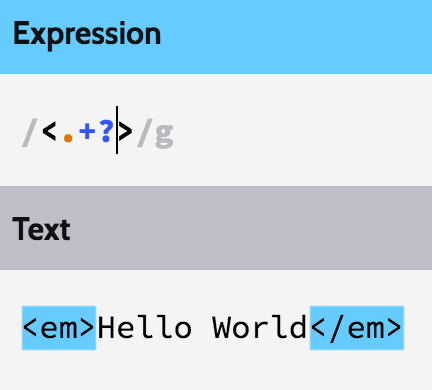
\includegraphics[width=.4\linewidth]{expr2}
    \caption{Lazy}
  \end{subfigure}
  \caption{Greedy vs. Lazy regular epxression \cite{regexr}}
  \label{fig:regexes}
\end{figure}

\subsection{Backtracking}
If the regular expression engine backtracks, the performance degrades. Backtracking is done when the engine matches at a different point in the pattern \cite{why-use}. Lazy quantifiers limit the amount of backtracking needed.

Example: \textsc{.+b}. If you want to match this to \textsc{aaaaaabcd}. You get the following trace:

\begin{itemize}
  \item aaaaaabcd
  \item aaaaaabc
  \item aaaaaab
\end{itemize}

This is an example of poor performance, which is illustrated by Figure \ref{fig:poorperf}.

\begin{figure}[b]
  \centering
    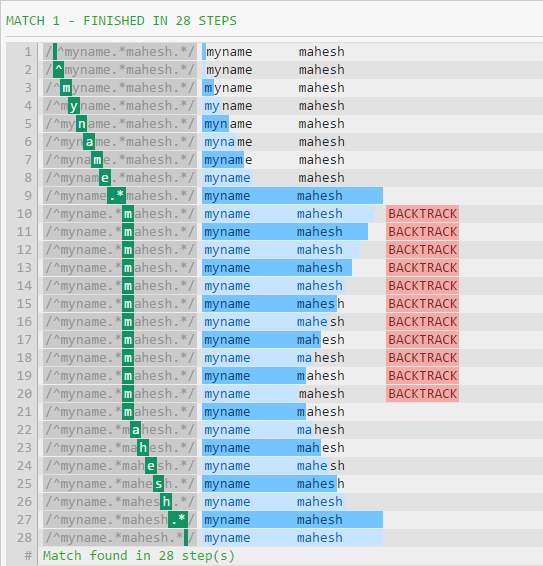
\includegraphics[width=.8\linewidth]{poorperf}
    \caption{Example of poor performance with backtracing \cite{regx101}.}
    \label{fig:poorperf}
\end{figure}

\subsection{Back referencing}
Notations vary. A few examples:

\begin{verbatim}
(abc|def)=\1 matches abc=abc or def=def, but not abc=def or def=abc \cite{refcapture}.

([a-c])x\1x\1 matches axaxa, bxbxb and cxcxc 3).

\b(\w+)\s+\1\b finds duplicate words that follow each other inside a document.
\end{verbatim}

\newpage
\section {The second week: \textit{GNU autotool}}
\newpage
\begin{thebibliography}{9}
  \bibitem{source1} 
    SamRuby. 
    \textit{intertwingly}. 
    RSS and Atom, reading, 2008.

  \bibitem{source2} 
    M. Nottingham 
    \textit{autocomplete-xml{\"o}rper}. (ATOM) 
    [\textit{Request for comment }]. 
    Network Working Group, 322(10):RFC4287, 2005.

  \bibitem{source3} 
    pleonex,
    \\\texttt{Autocomplete XML Atom Package/\~{}https://atom.io/packages/autocomplete-xml}
    
  \bibitem{url-regex-demo} 
    M. Bynens 
    \\\texttt{https://mathiasbynens.be/demo/url-regex}

  \bibitem{why-use} 
    M. Schulz
    \\\texttt{https://blog.mariusschulz.com/2014/06/03/why\\-using-in-regular-expressions-is-almost-never-what-you-actually-want}

  \bibitem{refcapture} 
    J. Goyvaerts
    \\\texttt{http://www.regular-expressions.info/refcapture.html}


  \bibitem{xpathwiki} 
    WikiPedia
    \\\texttt{https://en.wikipedia.org/wiki/XPath}
   \bibitem{regexr} 
    RegExr
    \\\texttt{http://regexr.com}
    
    \bibitem{regx101} 
    Regular Expressions 101
    \\\texttt{https://www.regex101.com/}
    
     \bibitem{w3c1}
    W3C
    \\\texttt{http://www.w3schools.com/xsl/xpath$_$intro.asp}

\end{thebibliography}
\end{document}
